%----------------------------------------------------------------------------------------
%	PACKAGES AND DOCUMENT CONFIGURATIONS
%----------------------------------------------------------------------------------------

\documentclass[a4paper,twoside,12pt]{report}
\usepackage[toc,page]{appendix}
\usepackage{booktabs}
\usepackage{graphicx} % Required for the inclusion of images
\usepackage{amsmath} % Required for some math elements
\usepackage[top=1.0in,bottom=1.0in,left=1.0in,right=1.0in]{geometry}  %bindingoffset=1in	 
\usepackage{float}
\usepackage[english]{babel}
\usepackage{hyperref}
%\usepackage{times}
\usepackage{setspace}
\usepackage{float}
\usepackage{subcaption}
\usepackage{graphicx}
\usepackage{mathptmx} %for times new roman
\usepackage{titlesec}
\usepackage{acro}

%----------------------------------------------------------------------------------------
%	TITLE DISPLAY
%----------------------------------------------------------------------------------------


\titleformat{\chapter}[display]
{\bfseries\Huge\centering}{\chaptertitlename\ \thechapter}{18pt}{\Huge}
\titleformat{\section}
  {\Large\bfseries}{\thesection}{12pt}{}
\titleformat{\subsection}
  {\large\bfseries}{\thesubsection}{11pt}{}

%----------------------------------------------------------------------------------------
%	INDEX, TABLE OF CONTENT, TABLE OF FIGURE, ACRONYM
%----------------------------------------------------------------------------------------


\begin{document}
\renewcommand{\contentsname}{Index}
\renewcommand{\bibname}{References}
\pagenumbering{roman}
\begin{spacing}{1.5}
\tableofcontents

\addcontentsline{toc}{chapter}{List of Tables}
\listoftables

\addcontentsline{toc}{chapter}{List of Figures}
\listoffigures

\chapter*{Acronyms}
\textbf{DNS} Domain Name System
\\*
\textbf{DNS} Domain Name System

\end{spacing}
%----------------------------------------------------------------------------------------
%	ABSTRACT
%----------------------------------------------------------------------------------------

\newpage
\addcontentsline{toc}{chapter}{Abstract}

\begin{spacing}{1}  %single spacing for abstract
\begingroup
\fontsize{12pt}{14pt}\selectfont
\begin{center}
	\Huge\bfseries
	\textit{Abstract}
\end{center}
\vspace{0.3in}
\textit{\fontsize{10}{10}\selectfont Blockchain has acquired popularity all over the world in a short period due to its distributed data management solution. Blockchain has provided security and data integrity with the intervention of the third party. One of the prominent use of blockchain technology is as a cryptocurrency. People are using cryptocurrency for transferring money, but it has also attracted hacker from all over the world. Attackers are targeting blockchain projects because of high investments. Since its early period of blockchain, there has been a series of attacks on the blockchain frame. In order to make understanding easy, the report contains a description of types of the network. In order to take a step towards solving this issue, the primary purpose of this report is to give detail about blockchain technology, how it is vulnerable to various kind of attack from the adversary. Public and private blockchain are detailed with their pros and cons. Apart from that, some non-technical risks are also discussed. This report also gives insights about some attacks on blockchain projects.   
\\*
\\*
\textbf{Keywords:} Blockchain Technology - Attacks - Risk - Prevention 
}
\endgroup
\end{spacing}
\begin{spacing}{1.5}
\chapter{Introduction}
Blockchain facilitates to transfer value without the need for an intermediate party. Examples of such values are information, contracts, assets, identity. This technology gives cryptographically secure and decentralized mechanism that removes the need for management from a single entity. Blockchain technology is building block for the cryptocurrencies such as Bitcoin and Ethereum. It is efficiently shared, trusted, and secure ledger of various transactions.  
\par
The traditional approach for payment methods and storage purposes are in a centralized manner. Trusted third party is required for electronic banking transaction. The intervention of the third entity makes transaction slower and expensive, and even high cost is needed to make an irreversible transaction. To tackle this issue,  a system required, which has unique features such as publicly available, free from the inference of the third party, irreversibility and secure. In October 2008, Satoshi Nakamoto published for peer-to-peer distributed technology which can fulfil all these requirements preciously. It uses cryptographic proof rather than a trusted third party, which enable two or more entities to participate directly. It enables to make transactions publicly available to read, which also hides the identity of a specific user. This advanced technology is secure as far as a single entity or organization does not control more than 50\% of network \cite{satoshinakamoto}. Immutability of ledger can be useful for saving data for a more extended period without risk of tamper. According to some experts, this technology has the potential to change the future of many industries.
\par
Blockchain has received popular all over the world in a short period. Researches are going on to use the benefits of blockchain in various field. However, like other technologies, blockchain is also vulnerable to threats and attacks from the adversary. As a result of that, researches for making blockchain immune to the attacks also started.         
\pagenumbering{arabic}
\section{Motivation}
Myriads of advantages have made blockchain one of omnipresent technology in recent time. However, the number of threats and attacks on this technology are increased. It has also attracted hackers to steal value and data, and because of that, many hacker's ground and attacker are finding new ways to find loopholes in the implementation of blockchain. In the past, they have even succeeded in many attempts, and users and organization have lost sensitive information and value worth of tremendous money.
\par
Famous cryptocurrency Verge has been a victim of cyber attacks for two times. The first attack was during April 2018, at that time attackers stolen digital coin worth of more than \$1.1 million. In May 2018, verge faced the same problem and lost around \$1.75 million \cite{verge_51_attack}. Just Dice was one of the most popular gambling platforms during the year 2013. Authorities announced that some stupid mistakes cost them for \$1,21,000 approximately 1,300 BTC at that time \cite{all_bitcoin_scam}. During November 2012, trojan horse virus was installed on user PCs, which resulted in the loss of 3,457 Bitcoins. Another blockchain technology, MyBitcoin lost almost \$2 million on $8^{th}$  August 2011 \cite{mybitcoin_hack}. 
\par
Apart from that, a blockchain start-up, The Backdoor, hacked its own wallet to save own users from possible attacks from attackers. Experts say that these attacks could have avoided with proper planning and preventive measure. Considering above mentioned losses and what happened with The Backdoor, it becomes vital to analyze potential attacks on blockchain framework. Analysis and adaption of preventive measure of such attacks and risk are also paramount. 
\section{Objective}
To give a lucid explanation of centralized, decentralized and distributed system, so that it becomes easy to understand important of blockchain and reason behind its popularity. This report also aims to explain the working and important features of blockchain. Types of blockchain, such as public blockchain and private blockchain, are also detailed.  
\par
A core objective of this report is to analyze various attacks, risk, issues and their prevention measure for the distributed ledger technology called Blockchain. It also aims to provide insights into examples, in which blockchain technology has been a victim of the malicious intention of attackers.
\section{Applications}
\subsubsection{Cryptocurrency}
Omnipresent digital currency mechanism facilitated by Blockchain works automatically, it also facilitates a real-time, time-efficient transaction which might be next to impossible in traditional database system \cite{overviewofblockchainsecurity,democraticmininginbitcoins}. Use of cryptocurrency removes the requirement of the third party, which makes the whole system fast and reliable. It also enables banks to progress payment speedily and more preciously while reducing resource requirements.
Address of each node is also a cryptographic hash, which can hide the identity of a particular node.  Various feathers provided by Blockchain makes it next-generation business process development.
\subsubsection{Supply Chain Use}
Suppliers can use blockchain for tracking products from the origin of the raw materials to the final products. Which will not only enables suppliers and manufacturers to verify the authenticity of the product, but also it will increase the trust of consumers for product and brand.
\subsubsection{Health Care}
Health care service providers can make the best use of blockchain, for securely saving data of their patients, types of equipment. Whenever a patient's record is generated, it can be digitally saved on the blockchain, which also provides proof and trust to the patients that record would not be altered in the nearby future. Furthermore, encoding can be used before saving record directly on the blockchain, which will intend to provide a level of security to any specific user. 
\subsubsection{For Voting System}
Use of blockchain in the voting system has the potential to remove the lurking risk of fraud in the voting process. During November 2018 in West Virginia, such voting system was tested even \cite{blockchain_in_voting}. In which, each vote can be considered as a block, making them infeasible to be altered. It can also bring transparency in the voting system, with that it can also provide the facility of the instant result.
\section{Report Outline}
In chapter \ref{chapter2}, the background of the problem is described, which includes types of system, working and features of blockchain with possible diagram. Types of blockchain, such as private and public, are also explored. Chapter \ref{chapter3} gives insights for possible attacks on blockchain and its preventive measure. Some non-technical risks are also explored.
\chapter{Background and Literature Survey}
\label{chapter2}
\section{Types of System}
Every system can be divided into three categories. First, centralized. Second, Decentralized and third is Distributed. Differences in the system can affect every whoever is using it \cite{gfg_cent_vs_decent}. Simultaneous use of these three categories is not possible. Hence, organizations and institutions need to choose out of available option. While deciding, which system to use, pros and cons of each system should be considered. With history's perspective, a centralized system is more prominent. But the centralized system has its disadvantages which can be overcome by a decentralized or distributed system. Below detail explanation of each system is given with its potential advantages and disadvantages.
\subsection{Centralized Framework}
Centralized system is more easy to define, implement and more intuitive. The centralized system uses typical client/server architecture, where an unlimited number of client-side nodes can communicate with one server-side node. Every client nodes are connect to server node, so server node can be considered as central node, and central node is responsible for working as storage from where every client can access their information. 
Wikipedia, IBM are centralized systems. In which, user can search for a specific query, and that query will be resolved by server lying at possibly any corner of the world.
\subsubsection{Advantages}
\begin{enumerate}
\item{Quick, easy deployment and quick development}
\item{Easy maintenance of system as whole}
\item{Feasible to control data from central entity}
\item{Cost effective}
\item{Quick update}
\end{enumerate}
\subsubsection{Disadvantages}
	\begin{enumerate}
	\item{Network connectivity is a key factor - Chances of system failure is higher, due to dependency on single server}
	\item{Longer access time for nodes residing at far points}
	\item{Difficult Server Maintenance because of only one server}
\end{enumerate}	 
\subsection{Decentralized Framework}
In this type of system, multiple central entities are available rather than single central entities, and these central entities are also connected to each other. Every central entity also stores an own copy of data. Presence of centralized still makes still vulnerable to an accident as a centralized one. However, the architecture of the decentralized system adds robustness, because even if the central entity fails, the rest of the central entities still continue to work. It means, it allows the system administrator to repair one central node, while the system itself continues its work, with limitation on performance and data availability to some extent.   
\subsubsection{Advantages}
\begin{enumerate}
	\item{Access time is faster than centralized system}
	\item{High fault tolerance}
	\item{More flexible and diverse system}
	\item{Scalability is higher than centralized}
	\item{Easy evolution}
\end{enumerate}
\subsubsection{Disadvantages}
\begin{enumerate}
	\item{Security and privacy risk}
	\item{Higher maintenance cost}
\end{enumerate}
\subsection{Distributed Framework}
The distributed system removes the need for a central entity, which ultimately rejects centralization. Each and user have equal access. However, access rights can be altered as when required. Blockchain and the internet are a well-known example of a distributed system. It is free from independent failure. Apart from that, it also allows the user to define ownership of data. Resources are distributed among users that lead to improved efficiency of the network. Because of the benefits it provides, the distributed framework is changing industry drastically.
\subsubsection{Advantages}
\begin{enumerate}
	\item{Transparency}
	\item{Scalable}
	\item{Easy evolution}
	\item{Extremely high fault tolerance}
\end{enumerate}
\subsubsection{Disadvantages}
\begin{enumerate}
	\item{Difficult to implement}
	\item{Higher maintenance cost}
\end{enumerate} 
\section{Blockchain Technology}
Blockchain is a chain of digital blocks containing various data and information. Once a block is connected to the chain, it can never be changed again, and it will be publicly available to read. For connecting the new block to the chain, blockchain uses the hash value of the previous block and new block. Digital blocks contain information of hash of the previous block, time and information which is to be added, etc. That is quite groundbreaking due to its avails facility for keeping track of medical records, full supply records and transaction records, etc. Some important terminologies are explained below.
\subsubsection{Nonce}
Blockchain allows the only specific type of hash values. For example, the first ten digits should be zero only. It is not always the case that the hash value will have ten-digit in starting. In order to, meet up this requirement while finding available signature data in the string needs to be changed continuously. Moreover, hash functions are designed in such a way that only a trivial change in a string can lead to the complete different hash value. So, a small special piece of data is added in the string to get an acceptable hash value. That piece of data is known as a nonce.   
\subsubsection{Mining Process and Miners}
\label{miningprocess}
The process of finding nonce is called mining. The entity which continuously works to find such nonces are known as miners. Methods that miners use can also be related to trial and error method. Miners use their computation power for finding an acceptable signature. Acceptable signature is expected output from any miner. Large computational power increases the possibility of finding out proper nonce in lesser time. In the case of publicly available blockchain, any user can work as a miner by using blockchain specific application. Process, in which, miners compete to get signature and get a reward for success is also known as Proof-of-Work \cite{satoshinakamoto}. The second method for choosing miner is called Proof-of-Stack. In Proof-of-Stack selection of miner depends on the cryptocurrency miner posses, rather than computational power which is used in Proof-of-Work \cite{saad_exploring_2019}. Other popular consensus algorithms are Practical Byzantine fault tolerance (PBFT), Proof-of-Reputation \cite{saad_exploring_2019}.
\begin{figure}[h!]
\begin{center}
  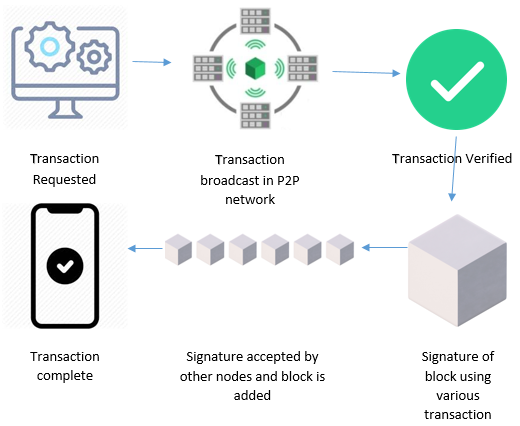
\includegraphics[width=0.8\linewidth]{images/workingofblockchain.png}
  \caption{\fontsize{10}{10}\selectfont Working of blockchain}
  \label{img: workingofblockchain}
\end{center}
\end{figure}  
\subsubsection{How Block is Added to ledger?}
According to Fig \ref{img: workingofblockchain}, whenever new data is to be added in blockchain, it is added into the imaginary pool of unverified data. Miners who have to participate in the mining process can access those data from the pool. Once miners get enough information that can create one block, they fetch data from the pool and start mining procedure as explained in section \ref{miningprocess}. As soon as miner find an acceptable signature, it broadcast that signature in the system. Agreement from the predefined percentage of a node is required. Once that many nodes agree for a new block, a new block is added to the ledger. Afterwards, the block becomes immutable.
%\section{Different Hash Function}
%\subsection{SHA-256} Bitcoin is using this. 
\section{Features of Blockchain Technology}
\subsection{Robustness}
Myriads of computers all around the world keep own copy of the ledger, and availability of duplicate copies makes Blockchain robust to the failure of single (or a few) node \cite{satoshinakamoto}. Unavailability or instability of node doesn't stop the whole system from working, because ledger still exists in other nodes. Alteration of data at one node is infeasible; it requires agreement or change in data on at least 50\% of the node.
\subsection{Censorship-Resistance}
Absence of a single entity which manipulates a blockchain that is a paramount feature of a decentralized network. In a centralized approach, one authority has access to the whole database, and it can change the database as and when required \cite{satoshinakamoto}. For example, while doing a bank transaction, the third party is always involved. On the other hand, blockchain abolishes interference of centralized authority, which facilitates to do the transaction directly between two parties.
\subsection{Transparency}
Each and every change in ledge also goes through every participant. Updates in the database are reflected in every node so that new information is available in little time. It means each node has knowledge about the data residing at another node. Data is also consistent with every node; it provides transparency to the system \cite{satoshinakamoto}.  
\subsection{Irreversibility}
Every transaction of the ledger in blockchain defines the next transaction. In other word, every transaction contains a hash value of the previous transaction. It means that every block of the chain is connected. So, for changing one block of the ledger, all the previous transaction requires changes, that is an infeasible task for today's computer. That characteristic makes blockchain irreversible and secure against a potential threat.
%\subsection{Security Purposes}
%\subsection{Time Constraint}
%\subsection{Financial Saving}
\subsection{Disaster Recovery}
Synchronized storage of data at various node improves the fault-tolerance and reliability of blockchain. Every node has access to create data and store ledger of blockchain, but it comes the cost redundancy \cite{democraticmininginbitcoins,minerevolutioninbitcoinnetwork}.   
Moreover, an attack on an individual node can't cause destruction to the whole system \cite{fangfangdai}. 
%\subsection{Tamper Proofing}
%\cite{fangfangdai}
\section{Types of Blockchain}
On the basis of who can assess and control the blockchain, this technology has two types of mechanism. First is permissionless blockchain is open for public use, whereas the second one is permission blockchain which allows an only limited number of users. Description and example of both types are explained below.       
\subsection{Permissionless Blockchain}
Permissionless Blockchain is also known as public Blockchain. The whole idea differs from the previous type. Any computer, with adequate technological requirements mandated by the network, can participate as a minor. As the name suggests, no other personal identity or machine authorization required to play the role of a minor. It allows anyone to read and participate in the system. When it is used as a part of cryptocurrency, at that time, having cryptocurrency is enough to allow any user to transact digital money. This model almost resembles the basic idea of blockchain technology given by Satoshi Nakamoto \cite{satoshinakamoto}. On the other hand, scalability and privacy issues are the drawbacks of a public blockchain. To conclude, any entity can participate for a transaction, and that can result in the privacy breach. Bitcoin and Ethereum are examples of permissionless blockchain technology. 
\subsection{Permissioned Blockchain}
Blockchain was originally developed as a publicly available and free system, but permission blockchain is exactly contrasting. Permission from the owner is required to take part in the blockchain. It gives control in the owner's hand, and it also means that one entity can manipulate the whole system. That right of possession allows authorities to do whatever want to do with the system, and also enables to impose various access rights to other users. For example, the owner can restrict some node from reading information. Even a validation procedure is done by only selected entities. That makes this model faster and scalable than public blockchain. As an epitome, USA based supermarket company Walmart is designing private blockchain to track fruits and vegetables. On top of it, some information regarding products will be publicly available. Moreover, a private blockchain is becoming popular in industries such as supermarkets, agriculture and transportation, and many more.
%\section{Current Research}
%\cite{fangfangdai}
\chapter{Cybersecurity Attacks, Risk and Prevention}
\label{chapter3}
\section{Types of Attacks and Prevention Measure}
\label{typesofattacks}
Attackers have stolen \$1 billion from cryptocurrency exchanges and various other platform \cite{topfiveblockchainsecurityissues}. It becomes vital to analyse such potential attacks which have affected users and validation nodes all over the world. The different methodology can be used for damaging blockchain, and various preventive measures are required to thwart the effect of malicious attack \cite{blockchainthreatreport}. 
\subsection{Phishing}
Phishing is defined as a malicious attempt to extracting information from users \cite{wiki:phishing}. It includes sensitive information such as bank details, username, password, etc. In short, phishing is stealing confidential data by masquerading attackers as a trusted party. Phishing breaks the confidentiality of information \cite{andryukhinphishing}. Email spoofing and messaging are prominent ways to expose any computer to this attack. For the implementation of phishing, attackers mostly disguise themselves as a representative of the reputed firm. In addition to that, attackers make their own website or application by a name trivially different from the original one. By the use of email or message, the address of this platform is sent to a potential victim. For example, an institute called Block.one which developed EOS.IO blockchain during 2018, has been the victim of phishing attack \cite{wiki:phishing}. Phishing group sent an email with the intention of stealing wallet key. Unfortunately, an attack was successful. 
\par
Clone phishing is a type of attack in which duplicate webpage with also most resembling, or webpage with approximately same is made \cite{andryukhinphishing,phishingkaspersky}. Targeted phishing one of the prominent type of attack. It includes aiming at owners of wallets, the key person of companies, and owner of cryptocurrency \cite{aimedphising,andryukhinphishing}. Duplicate cryptocurrency purses uses forgery purse, in which applications related to cryptocurrency is published on a well-known application providing platform. Then that malicious demands for the private key and purse password \cite{andryukhinphishing}.          
\subsubsection{Electrum Bitcoin}
Electrum bitcoin wallet has been a victim of a phishing attack. From December 2018 to April 2019, Electrum bitcoin wallet user lost almost \$4 million which is as equal as around 771 BTC for the month of April of 2019
\cite{phishing_perez_behind_2019}. Research is done by Malwarebytes Labs, and attackers successfully tricked wallet owners into downloading fraudulent version of the wallet.  
\subsubsection{How to Protect System From Phishing ?}
Modern methods for protecting the blockchain from phishing attack is related can be derived by the use of machine learning and artificial intelligence \cite{blockchainthreatreport,andryukhinphishing}. A large number of algorithms are being discovered to find out phishing sites.
\begin{enumerate}
	\item{One of the solutions finds an alternative of DNS, as an epitome, ENS (the Ethereum name Service) \cite{andryukhinphishing}.}
	\item{For the avoidance of attack on social networking sites, clone solution is to track the activity on corporate pages and community pages \cite{andryukhinphishing}.}
	\item{Surveillance of site traffic, avoiding risky transaction and investments come under  the ways to protecting system phishing.}
	\item{Verification of each sender's and receiver's address each time}
	\item{It is advisable not to open the suspicious link and not to download unknown attachments}
	\item{Authentication of SSL certificate before using any service}
	\item{Adapting two-step verification process}
	\item{Avoidance of public Wi-Fi}
\end{enumerate}  
\subsection{51\% attack}
\label{51attack}
Satoshi Nakamoto mentioned possible security attack on the blockchain by dishonest note \cite{satoshinakamoto}. For adding a block of unconfirmed transactions in the blockchain ledger, mining node needs to solve complex problems which require high computation power. Still, by controlling more than half of the blockchain framework, the attacker does harm to the framework. If more than 50\% of the network's mining power agree on wrong information, then incorrect information is considered as truth, and it becomes eligible to be added into a ledger. In another word, one entity control more than half of the system, then only that entity is sufficient to decide whether to allow transaction or not. Moreover, an entity will have the power to halt other transaction being added to the system. In a nutshell, one entity can monopolise the whole blockchain framework. Though 51\% attack can give control to the one entity, alteration of the early written block is still an infeasible task. The reason behind this is attacker would need to change the whole chain of the block, which is joined via a hash function. If 51\% attack is considered as a controlling framework without taking consideration of fraction of network which is under control, then 51\% attack is also possible for less than 50\% of mining power. But chances of getting success decreases. That security flaw also lies in cryptocurrencies such as Ethereal, Bitcoin Gold, Monacoin, Verge, and even gone through such attack, and almost \$20 million were stolen because of this type of attack during the period of 2016-17 \cite{topfiveblockchainsecurityissues,51attackonline}.

\subsubsection{Ghash.IO}
Ghash.IO operated during the year 2013-2016. By mining bitcoin worth of \$200 million during its first year, Ghash.IO showcased its tremendous mining power \cite{wiki:ghash.IO}. Because of this excessive hash rate, Ghash.IO was in controversy during the year 2014. It's mining power crossed the 50\% hash rate of the whole bitcoin, but then after Ghash.IO declared that it would exceed than 40.00\% \cite{wiki:ghash.IO}. 
\subsubsection{Krypton Framework}
Ethereum Krypton blockchain also suffered from 51\% attack. Attackers took two approaches to damage system. First was overpowering the framework with at least 50\% of hashing power, because of that they were able to roll back the transaction and spend coins twice. Attackers also launched a DDoS attack on Krypton's biggest mining pool, ensuring that the network was weak the time of the attack. Though amount which was stolen was around \$4,000  only, attack on Krypton Framework can't be ignored \cite{51attackonethereum}. This attack also comes under the category of double-spending and DDoS.
\subsubsection{Bitcoin Gold}
According to the experts, total \$18 million was stolen by a combination of both double-spending attack and 51\% attack \cite{51attackonbitcoingold}. Attackers used Bitcoin gold for the exchange of another coin, then they withdrew. Then again, they used coin from a wallet, means double-spending. 
\subsubsection{Protection of Blockchain Framework From 51\% Attack}
In order to counter this attack, one way is to change the number of confirmations required to confirm transaction \cite{what_is_51attack_2018}. Bitcoin and Krypton implemented this way in the past to get rid of 51\% attack.
\begin{enumerate}
	\item{Use of \textbf{delayed Proof-of-Work (dPoW)} which is updated consensus algorithm \cite{51_solution_2018}. In delayed Proof-of-Work, "delayed function" penalizes miner who might be preparing for such an attack. According to co-Founder of Horizen Rob Viglione, a delay function poses excessive cost, a 10x cost, which can make prohibitively expensive.}
\end{enumerate}
\subsection{DNS Redirection}
\label{dnsattack}
In order to steal sensitive information username, id and password. Most notorious way to do so is via DNS redirection. DNS redirection is also known as DNS hijacking. As shown in Fig \ref{img: dns}, this attack is performed by sending the wrong IP address to the user's computer, when the computer tries to resolve URL. Because of manipulated IP address, the user will be forced to visit a website other than expected. That website might resemble as the authentic one, due to that, it is very likely that the user will enter sensitive information such as username, password, bank details, etc. DNS redirection is one type of technical phishing \cite{andryukhinphishing}.
\begin{figure}[h!]
\begin{center}
  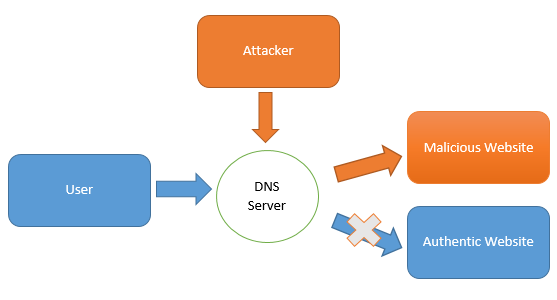
\includegraphics[width=0.8\linewidth]{images/dns.png}
  \caption{\fontsize{10}{10}\selectfont DNS attack}
  \label{img: dns}
\end{center}
\end{figure}
\subsubsection{BlackWallet.co}
On $13^{th}$ January of 2018, BlackWallet.co suffered from DNS Redirection attack. Adversaries redirected, the DNS entry of the BlackWallet.co domain, to a server they operated \cite{blackwallet_nodate}. As a result of that users were logging in malicious server, then attackers used that credentials to steal money from authentic wallet. Users lost around 6,70,000 Lumens which is one of the top ten cryptocurrency, contemporary worth of \$0.4 million. 
\subsubsection{Caution Against DNS Attack}
It is very difficult for normal user to interpret and confirm whether organization's DNS is hijacked or not, but as a active user, everyone can keep eyes on changes in website, application and unnecessary pop-up. 
\begin{enumerate}
	\item{Whenever a user accesses any website, the user can verify the certificate. It is preferable not to continue just because the URL is correct.}
	\item{Organizations should post security-related alert message on the website to make users aware of potential threat to the system.}
\end{enumerate}
\subsection{DoS Attack}
Traditional domain name resolution method uses a hierarchical resolution process, and the central server plays an important role. That makes the system most vulnerable to attack such DoS. In DoS (Denial of Service), adversary tries to make network, framework or system unavailable for indefinitely with the intention of disruption in system \cite{chao-yang_dos_2011}. In most of the cases, this attack is made by doing an excessive number of requests to the system, which can prevent query or request from authentic users \cite{dos_wireless_singh_denial_2017}. Well-known example of this attack is sending request to web server, which might result into the congestion in network and repudiation of request from some user. Such attack has a potential to damage blockchain framework also. For an example, a scenario in which nodes with malicious intention is part of network also. Now, malicious node can create unnecessary traffic in system. But it is very rare and difficult task in blockchain because of blockchain's dynamic topology \cite{zaghloul_beginners_2018}. In some cases, attackers use more than one node to send request in order do distributed attack, which is also known as DDoS \cite{saad_exploring_2019}. 
\subsubsection{Step Against DoS Attack}
Possibility of DoS can't be removed completely. However, there are some possible ways which can be used to curb DoS attack. Security of blockchain lies in the hashfunction with which blocks are related. 
One way to make blockchain secure is to reduce the size of block, but as size of block decreases number of transaction contained by single block also decreases. For security purpose, reducing the size of block is preferable. More number of block also increases transaction fees, that can be used to prevent DoS attack at some extent. Because while generating undesirable traffic on network, malicious nodes need to pay fees for each transaction. Size of block is parameters of the blockchain framework, by changing other parameters of the blockchain DoS attack can be controlled. Actually that method is trial and error method, researches are going on to find optimal result \cite{zaghloul_beginners_2018}. Penalizing nodes that sends lots of duplicate, expired, incorrect signature, so those nodes would get banned. Ultimately, DoS attack is inevitable, but certainly ,by proper care chances of success can be reduced at large extent.       
\subsection{Sybil Attacks}
Sybil attack is kind of attack in which one person or entities tries to control whole network by pretending to many users at same time, this can be done by creating multiple account, nodes or computers \cite{zaghloul_beginners_2018}. In simple language, it can be compared to making multiple social media accounts. For the crytocurrency, relevant example for this attack is to make multiple nodes of blockchain network. One way to exploit sybil attack is that attacker can always refuse to broadcast and transaction from any one the node, as a result of that it may isolate node from network. In fact, large-scale sybil attacks, where attackers tries control most of the network is known as 51\% attack. 51\% is explained in section \ref{51attack}.
\subsection{Eclipse Attack}
For an example, if given node is dependent on x number of node for its own view of distributed ledger. However, if adversary any how can manage to make the node to choose those x number of nodes from his/her malicious nodes alone, then he can eclipse the correct view of distributed ledger. In other words, attackers will control all the nodes to which given specific node is connect in given network, then attacker will successfully shows wrong ledger to the node, which will waste computation power of that peer.   	 
\begin{figure}[h!]
\begin{center}
  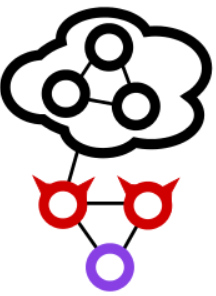
\includegraphics[width=0.3\linewidth]{images/eclipseattack.png}
  \caption{\fontsize{10}{10}\selectfont Eclipse attack}
  \label{img: eclipse}
\end{center}
\end{figure}
\\*
Fig \ref{img: eclipse}, depicts the possible scenario for eclipse attack. In figure block nodes shows legitimate blockchain network. Purple color shows targeted node, and red color denotes nodes which are controlled by attackers. From the Fig \ref{img: eclipse}, it is obvious that attacker has isolated victim node, and it may lead to display manipulated ledger to the victim node.  
\subsection{Selfish Mining Attack}
Blockchain's consensus algorithm allows only longest chain to be the trusted and correct ledger. It might reject correct ledger, if at all, it would be shorter than a corrupted one. This feature lead to the vulnerability in blockchain framework. Attacker might create its own fraudulent ledger, once it get longer than the correct, at least by one or two block, attacker will publish it, all over the network. Because of design of consensus algorithm, other node will accept that corrupted ledger as a authentic one. Just before publishing ledger on network, if attacker will do any transaction, then risk of double-spending is also there.
%\subsection{Exchange Hack}
%\cite{blockchainthreatreport}
%\subsection{Orphaned blocks}
%\cite{saad_exploring_2019}
%\subsection{Eclipse Attack}
%\cite{saad_exploring_2019}
%\subsection{Consensus Delay}
%\cite{saad_exploring_2019}
%\subsection{Double-Spending}
%\cite{saad_exploring_2019}
%\subsection{Software Flaw}
%\section{Security Issues}
%Distribution of information and data among several computers residing at various locations removes %possibility of single node failure. In addition to that, use of ledger and hashing eliminates the issue of %hacking \cite{topfiveblockchainsecurityissues}. But, as mentioned below, Some issues are required to be taken %care, otherwise it might lead to repercussion.
%\subsection{Technical Limitations}
%Main idea of blockchain lies in storing redundant data at more one node. For the continuous updation is %mandatory, but for that complex network among participants.  
%\cite{fangfangdai}
%\subsection{Opensource BlockChain Platforms Attract Intensive Attacks}
%\cite{fangfangdai}
%\subsection{Security Management of Self-organization and Anonymity}
%\cite{fangfangdai}
\section{Security Risk}
Popularity and execution of any technology in industry relies on the effective risk management. Risk management becomes vital when Technology is core of the company. Blockchain is not an exception from them. Blockchain should be implemented correctly and effectively, so that it fulfills organization intention of data security, privacy, confidentiality and time efficient solutions.
\subsection{Standard Risks}
Organizations are vulnerable to the some standard risk even while using blockchain Technology. Such issues should be addressed for the efficient and successful use of blockchain \cite{securityrisk}. Below details about such typical risks are mentioned. 
\subsubsection{Planning Risk}
Resources, used for the implementation of blockchain, can be hindrance for the product and services being delivered from the platform of blockchain. In addition to that, organization should be careful while deciding which entities can participate in blockchain network. Because number of participation can create impact on the efficiency and security of blockchain.    
%\subsubsection{Business Continuity}	
\subsubsection{Reputational}
Most of the fintech applications of other technology are not the core of organization, whereas blockchain is heart for expansion and survival of institute. Failure of blockchain might leads to shut down of whole industry, and bad consumer experience.   
\subsubsection{Information Security Risk}
Firstly, as explained in \ref{typesofattacks}, blockchain is vulnerable to various cyberattacks such as 51\% attack, phishing, DNS hijacking, etc. 51\% attack is mostly dangerous for permissioned system. Secondly, user details such log in credentials, password is susceptible for attackers, who intent to take over user's account for malicious purpose. 	
\subsubsection{Technical Limitations}
Main idea of blockchain lies in storing redundant data at more one node. For the continuous updation is mandatory, but for that complex network among participants. It requires large scale network with huge computation power \cite{fangfangdai}.
\subsubsection{Regulatory}
In present, there is no regulatory compulsion for blockchain. But in the future, regulatory risk related is possible, such as whether to include international transaction or not, privacy and data protection concern for international transaction.    
\subsubsection{Operational and IT}
Current rule, regulations, procedure, law and policies needs to be changed to adapt new business methodology. In addition to that, there remains technological concern for catch up the demand of scalability and speed.   
%\subsubsection{Contractual}
%\subsubsection{Supplier}
\subsection{Value Transfer Risks}
Elimination of third party exposes communicating nodes to new risks, earlier these risks were controlled by trusted third party. In other word, there remains risk while transferring value from one node to another node. These value can be information, assets, and identity.
\subsubsection{Consensus Protocol}
The transfer of value between node occurs by agreement from other nodes which use consensus protocol, and
Proof-of-Stack and Proof-of-Work are consensus algorithms. Proof-of-Stack is consensus algorithm with the advantage of energy efficiency and security over Proof-of-Work \cite{saad_exploring_2019}. Deficient consensus protocol can lead to the fatal result. For an example, in the case of Proof-of-Stack, there is a chances of  problem called Nothing at Stack \cite{wiki:proofofwork}.  
\subsubsection{Data Confidentiality}
In distributed ledger technology, to fulfill the demand of system, data or information needs to be shared all over the network. Doing so result into the loss of confidentiality from basic requirements CIA (Confidentiality, Integrity and Availability). Monitory the metadata can revel a lot about the type of activity and volume associated with the activity of any public address.
\subsubsection{Key Management}
Though mechanism of blockchain makes it next to impossible to alter the block, chances of theft is private key is always there. Once private is exposed to the adversary, he/she can extract money using public key. So, when it comes blockchain's private key, precious and proper management of key becomes mandatory.
%\subsubsection{Assets}
%\cite{infinance}
%\subsection{Smart Contract Risks}
%\subsubsection{Business and Regulatory}
%\subsubsection{Legal Liability}
%\subsubsection{Enforcement of contract}
%\subsubsection{Information Security}
\chapter{Conclusion}
Table \ref{tab:relationattackancomponent} shows which types of attacks can harm which component of blockchain framework. Presence of bullet shows the high possibility. For an example, DNS hijacking can effect Users, because as explained in section \ref{dnsattack}, user can be redirected to fallacious website.   
\label{chaper4}
\begin{table}[h!]
  \begin{center}
    \caption{\fontsize{10}{10}\selectfont Relations Between Various Attacks and Component of Blockchain Framework}
    \label{tab:relationattackancomponent}
    \begin{tabular}{l|c|c|c|c|c} % <-- Alignments: 1st column left, 2nd middle and 3rd right, with vertical lines in between
      \toprule
      \textbf{} & \textbf{Blockchain} & \textbf{Miners} & \textbf{Mining Pools} &\textbf{Exchange} &\textbf{User}\\
		\hline
      DNS hijacking         &         &$\bullet$&$\bullet$&$\bullet$&$\bullet$\\
		\hline      
      DoS                   &$\bullet$&$\bullet$&$\bullet$&         &\\
		\hline      
      51\% Attack           &$\bullet$&$\bullet$&         &         &\\
		\hline      
      Phishing              &         &$\bullet$&$\bullet$&$\bullet$&$\bullet$\\
		\hline
	  Eclipse Attack        &         &$\bullet$&         &         &$\bullet$\\
      \hline
	  Selfish Mining Attack &$\bullet$&$\bullet$&$\bullet$&         &\\
      \bottomrule
    \end{tabular}
  \end{center}
\end{table}
%\begin{appendices}
%\end{appendices}

%----------------------------------------------------------------------------------------
%					Bibliography
%----------------------------------------------------------------------------------------
\end{spacing}
\bibliography{report}
\addcontentsline{toc}{chapter}{References}
\bibliographystyle{ieeetr}
\begin{spacing}{1.5}
\chapter*{Acknowledgement}
I take this opportunity to express my deep sense of gratitude and indebtedness to my seminar guide, Dr. Sankita J Patel , my seminar coordinator Mr. R. P. Gohil and H.O.D, Dr. M. A. Zaveri from Computer Engineering Department, SVNIT Surat for their valuable guidance, useful feedback and co-operation with kind and encouraging attitude towards this seminar.
\end{spacing}
\end{document}

